%Author: Martiano Jimenez
%Date: 30.December.2024

\documentclass[11pt]{beamer}
\usetheme{Darmstadt}
\usepackage[utf8]{inputenc}
\usepackage[spanish]{babel}
\usepackage{amsmath}
\usepackage{amsfonts}
\usepackage{amssymb}
\usepackage{graphicx}
\author{Ing. Mariano Jim\'enez Brenes}
\title
{
E2025C2-G01-ELECTRÓNICA DIGITAL Y SEMICONDUCTORES.
}
%\setbeamercovered{transparent} 
%\setbeamertemplate{navigation symbols}{} 
\logo{
\includegraphics[height=0.75cm]{./images/castrocarazo.eps}\vspace{5pt}} 
\institute{
Universidad Castro Carazo\linebreak
T\'ecnico En Semiconductores
} 
\date{Mi\'ercoles 04.Junio.2025} 
%\subject{} 
\begin{document}

\begin{frame}
\maketitle 
\end{frame}

% Remove logo from the next slides
\logo{}

\begin{frame}
\frametitle{Contenido}
\tableofcontents
\end{frame}


\section{Electr\'onica Digital}
\subsection{Circuitos digitales y el
contexto de su evoluci\'on
tecnol\'ogica}
\begin{frame}{Circuitos digitales}
\frametitle{Circuitos digitales}
Electr\'onica:
	\begin{itemize}
		\item Procesamiento de datos... digital
		\item Transmisi\'on y Recepci\'on de datos... digital
	\end{itemize}
	¿Qu\'e noci\'on tenemos de los Sistemas digitales y n\'umeros binarios?
\end{frame}
\subsection{Presentaci\'on Personal}
\begin{frame}{Presentaci\'on personal}
\frametitle{Presentaci\'on personal}
Alg\'un detalle personal que nos caracterice....
\end{frame}
\subsection{Acuerdo de Aprendizaje}
\begin{frame}{Acuerdo de Aprendizaje}
\frametitle{Acuerdo de Aprendizaje}
Revicemos las 30 sesiones de este cuatrimestre
\end{frame}


\section{Sistemas Num\'ericos}
\begin{frame}{Sistemas Num\'ericos}
\frametitle{Sistemas Num\'ericos}
	\begin{itemize}
		\item Representaci\'on de numeros decimales(10 s\'imbolos):\linebreak
			\linebreak
			\makebox[\textwidth][s]{$10^{3}a_{3}+10^{2}a_{2}+10^{1}a_{1}+10^{0}a_{0}+10^{-1}a_{-1}10^{-2}a_{-2}+10^{-3}a_{-3}$}
			\linebreak
		\item 
			Representaci\'on de numeros binarios(2 s\'imbolos):\linebreak
			1101.11
		\item 
			Representaci\'on de numeros octales(8 s\'imbolos):\linebreak
			72.11
		\item 
			Representaci\'on de numeros hexadecimales(16 s\'imbolos):\linebreak
			B1F.1C
	\end{itemize}
\end{frame}

\begin{frame}{Ejercicios}
\frametitle{Ejercicios de sistemas num\'ericos}
Ver ejercicios del 1.7 al 1.10 del Morris Mano.
\end{frame}

\section{Tablas de Verdad}
\begin{frame}{Tablas de Verdad}
\frametitle{Tablas de Verdad}
\begin{figure}[h]
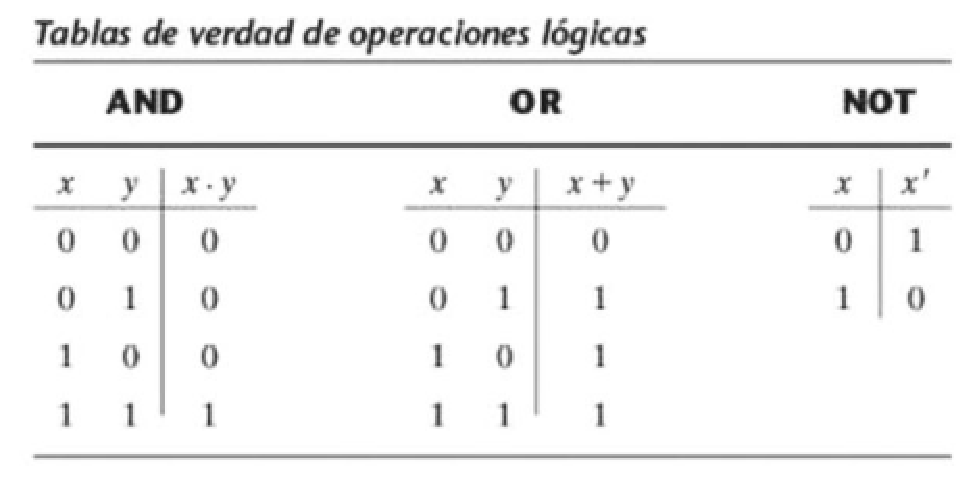
\includegraphics[height=3.0cm]{./images/tt.eps}\vspace{1pt}
\end{figure}
\end{frame}

\section{Diagramas de Temporizaci\'on}
\begin{frame}{Diagramas de Temporizaci\'on}
\frametitle{Diagramas de Temporizaci\'on}
\begin{figure}[h]
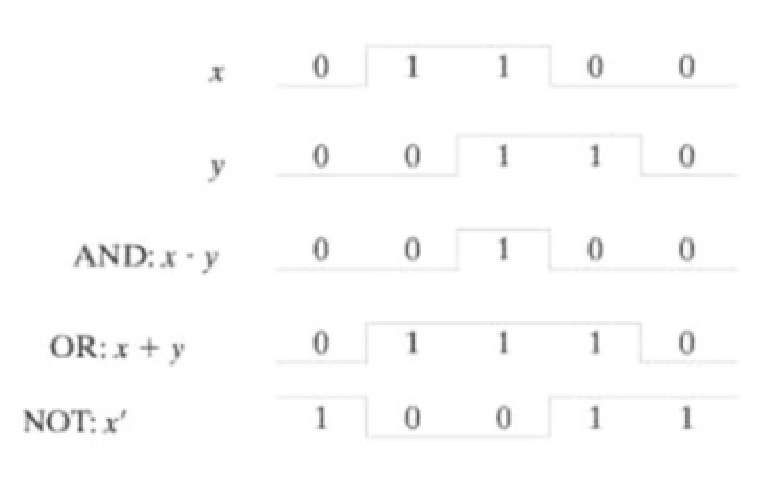
\includegraphics[height=3.0cm]{./images/td.eps}\vspace{1pt}
\end{figure}
\end{frame}

\begin{frame}
\frametitle{Ejercicios}
Realice los ejercicio del 1.34 \& 1.35 del Morris Mano y adicionalmente elabore las tablas de verdad de los circuitos que ah\'i se presentan.
\end{frame}

\section{Actividades Asincr\'onicas}
\begin{frame}
\frametitle{Actividades Asincr\'onicas}
	\begin{itemize}
		\item Elaboraci\'on de Documento:Utilizando el formato de art\'iculo para $IEEE$, realice y suba el informe sobre simplificación de funciones booleanas en un circuito secuencial.
		\item Indagaci\'on: Utilizando la AI investigue y comente en el foro sobre los circuitos integrados CI7410 NAND de 2 entradas Y CI 7420 NAND de 4 entradas 7402.
		\end{itemize}
\end{frame}

\section{Bibliograf\'ia}
\begin{frame}
	\frametitle{Bibliograf\'ia}
	\begin{itemize}
		\item Morris, M., y Ciletti, M. Diseño Digital, Cap. 9, pág. 446-448.
		\end{itemize}
\end{frame}

\end{document}